\chapter{Metodologia}

A metodologia deste trabalho foi dividida em duas partes: A obtenção dos dados da câmera, bem como \textit{keypoints} e \textit{keyframes} partindo da câmera de um \textit{smartphone} utilizando um aplicativo de autoria própria, o \textit{PhotoGuide}; e a reconstrução do ambiente utilizando a ferramenta \textit{LSD-SLAM}. O \textit{PhotoGuide} não foi usado na segunda parte do projeto devido à baixa performance e do baixo suporte nativo da ferramenta \textit{OpenCV} para \textit{Android} fazendo a reconstrução 3d ser migrada do \textit{smartphone} para uma ferramenta \textit{desktop}.


\section{\textit{PhotoGuide}}

Desenvolvido para a plataforma \textit{Android}®, o \textit{PhotoGuide} \cite{PhotoGuide} teve como objetivo primário a reconstrução de ambientes à partir da câmera do dispositivo que fosse executado da plataforma \textit{Android}. O aplicativo utiliza diversos algoritmos providos pela biblioteca de terceiros \textit{OpenCV} \cite{OpenCV}. O objetivo do \textit{PhotoGuide} é, partindo do \textit{stream} da câmera ou recebendo um conjunto de imagens sequenciais, obter os quadros num intervalo pré-determinado e então enviar pares para serem processados utilizando o \textit{ORB}, retornando os keypoints encontrados depois de filtrados, sendo inseridos num banco de dados no final do processo.  Primeiramente foi necessário obter os keypoints da cena, e os algoritmos mais utilizados para isso são \textit{SIFT} e \textit{SURF}, mas infelizmente ambos são patenteados, o que nos obrigaria a lidar com a questão das patentes e permissão de uso. O \textit{ORB} e \textit{BRISK} são algoritmos para obter keypoints e seus descritores, e foram desenvolvidos para terem uma performance semelhante ao \textit{SIFT} e\textit{ SURF}, tornando-se assim a melhor escolha já que são de livre uso.

Primeiramente, os \textit{keypoints} são obtidos diretamente da câmera do aparelho, mas a taxa de captura usada foi 10 quadros por segundo, e passados (como imagens \textit{bitmap} e em pares) para o \textit{ORB}; então são processado os \textit{keypoints} e seus descritores, mas infelizmente é possível haver ruído na imagem e, portanto, ocasionando em falsos casamento entre uma imagem e outra. Para remover o máximo possível de falsos positivos, foram utilizadas três técnicas de refinamento, na ordem: \textit{Cross Check}, \textit{Ratio Filtering} e \textit{RANSAC}.

Ao executar o \textit{ORB} e \textit{BRISK}, são obtidos listas de estruturas que possuem informações acerca do keypoint, bem como informações sobre seu correspondente na segunda imagem. O \textit{Cross Check} consiste em rodar o algoritmo duas vezes, uma procurando pontos da primeira imagem na segunda, e outra vez procurando pontos da segunda imagem na primeira. Por fim, percorre ambos, verificando se para cada casamento da primeira lista, as informações batem com o casamento correspondente da segunda lista.

O \textit{Ratio Filtering} percorre a lista resultante, verificando se há mais de um casamento para cada \textit{keypoint}, já que o ideal é que cada \textit{keypoint} tenha apenas um único correspondente na segunda imagem. Ao encontrar mais de uma ocorrência, descarta os pontos mais distantes.

Por fim, a ultima filtragem é realizada com o \textit{RANSAC} \cite{RANSAC}. O \textit{RANSAC} é um método iterativo para estimar parâmetros de modelos matemáticos partindo de um conjunto de informações obtidas que possuem \textit{outliers}. Também é considerado um método determinístico que possui um bom resultado com confiabilidade. Foi apresentado em 1981 por Fischler e Bolles para tentar resolver o problema da determinação da localização. Ele parte do principio que o conjunto de informações possui inliners, os quais são informações que podem ser explicadas pelos parâmetros do modelo, apesar que podem ter sofrido de ruido, e os outliers, que são informações que não condizem com o modelo. Esses \textit{outliers} podem ser provenientes de ruido, medições errôneas ou uma má interpretação das informações. A figura \ref{fig3:1} possui um exemplo de um conjunto de informações, os pontos, e como o \textit{RANSAC} trataria os \textit{inliners} e \textit{outliners}:

\begin{figure}
	\centering
		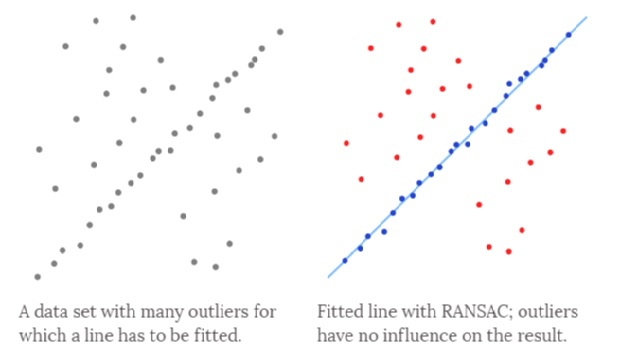
\includegraphics{Imagens/figura3-1.jpg}
	\caption{Exemplificação do tratamento do \textit{RANSAC} com os \textit{inliners} e \textit{outliners}. Imagem licenciada pela CC 3.0}
	\label{fig3:1}
\end{figure}
  

Por fim, as comparações entre as imagens eram retornadas, e seus \textit{keypoints} armazenados num banco de dados, para futuro processamento, a figura \ref{fig3:2} mostra um exemplo da execução do app:

\begin{figure}[H]
	\centering
		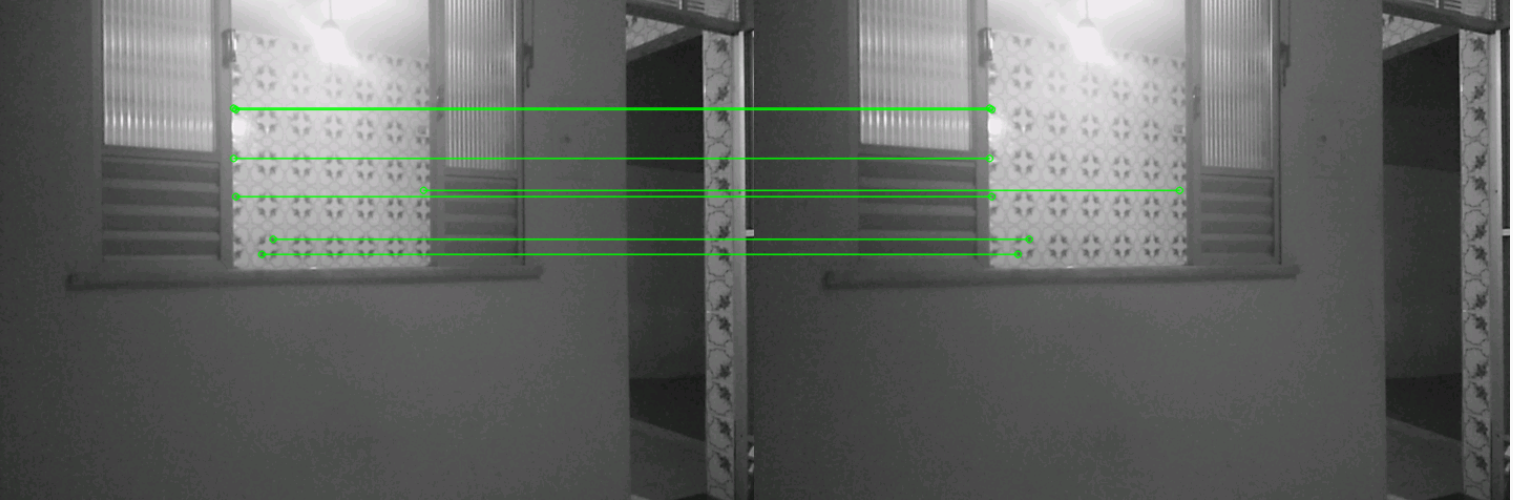
\includegraphics[width= \textwidth]{Imagens/figura3-2E4-4.png}
	\caption{\textit{Keypoints} encontrados e filtrados entre duas imagens.}
	\label{fig3:2}
\end{figure}

 
Foi adicionado ao aplicativo a opção de realizar a calibração da câmera com o auxílio da biblioteca \textit{OpenCV}, já que foi percebido que a distorção radial da câmera estava influenciando os resultados. A calibração da câmera, numa forma prática, consiste em fornecer um \textit{stream} da câmera ou sequência de fotos, contendo um padrão pré-definido. O \textit{OpenCV} fornece funções para calibrar a câmera de um dispositivo, necessitando das imagens capturadas do padrão, dentre as seguintes opções:

\begin{itemize}
	\item{Tabuleiro de xadrez em \ref{fig3:3}}
	\item{Círculos alinhados assimetricamente \ref{fig3:4}}
	\item{Círculos alinhados simetricamente \ref{fig3:5}}
\end{itemize}

\begin{figure}[H]
\minipage{0.32\textwidth}
  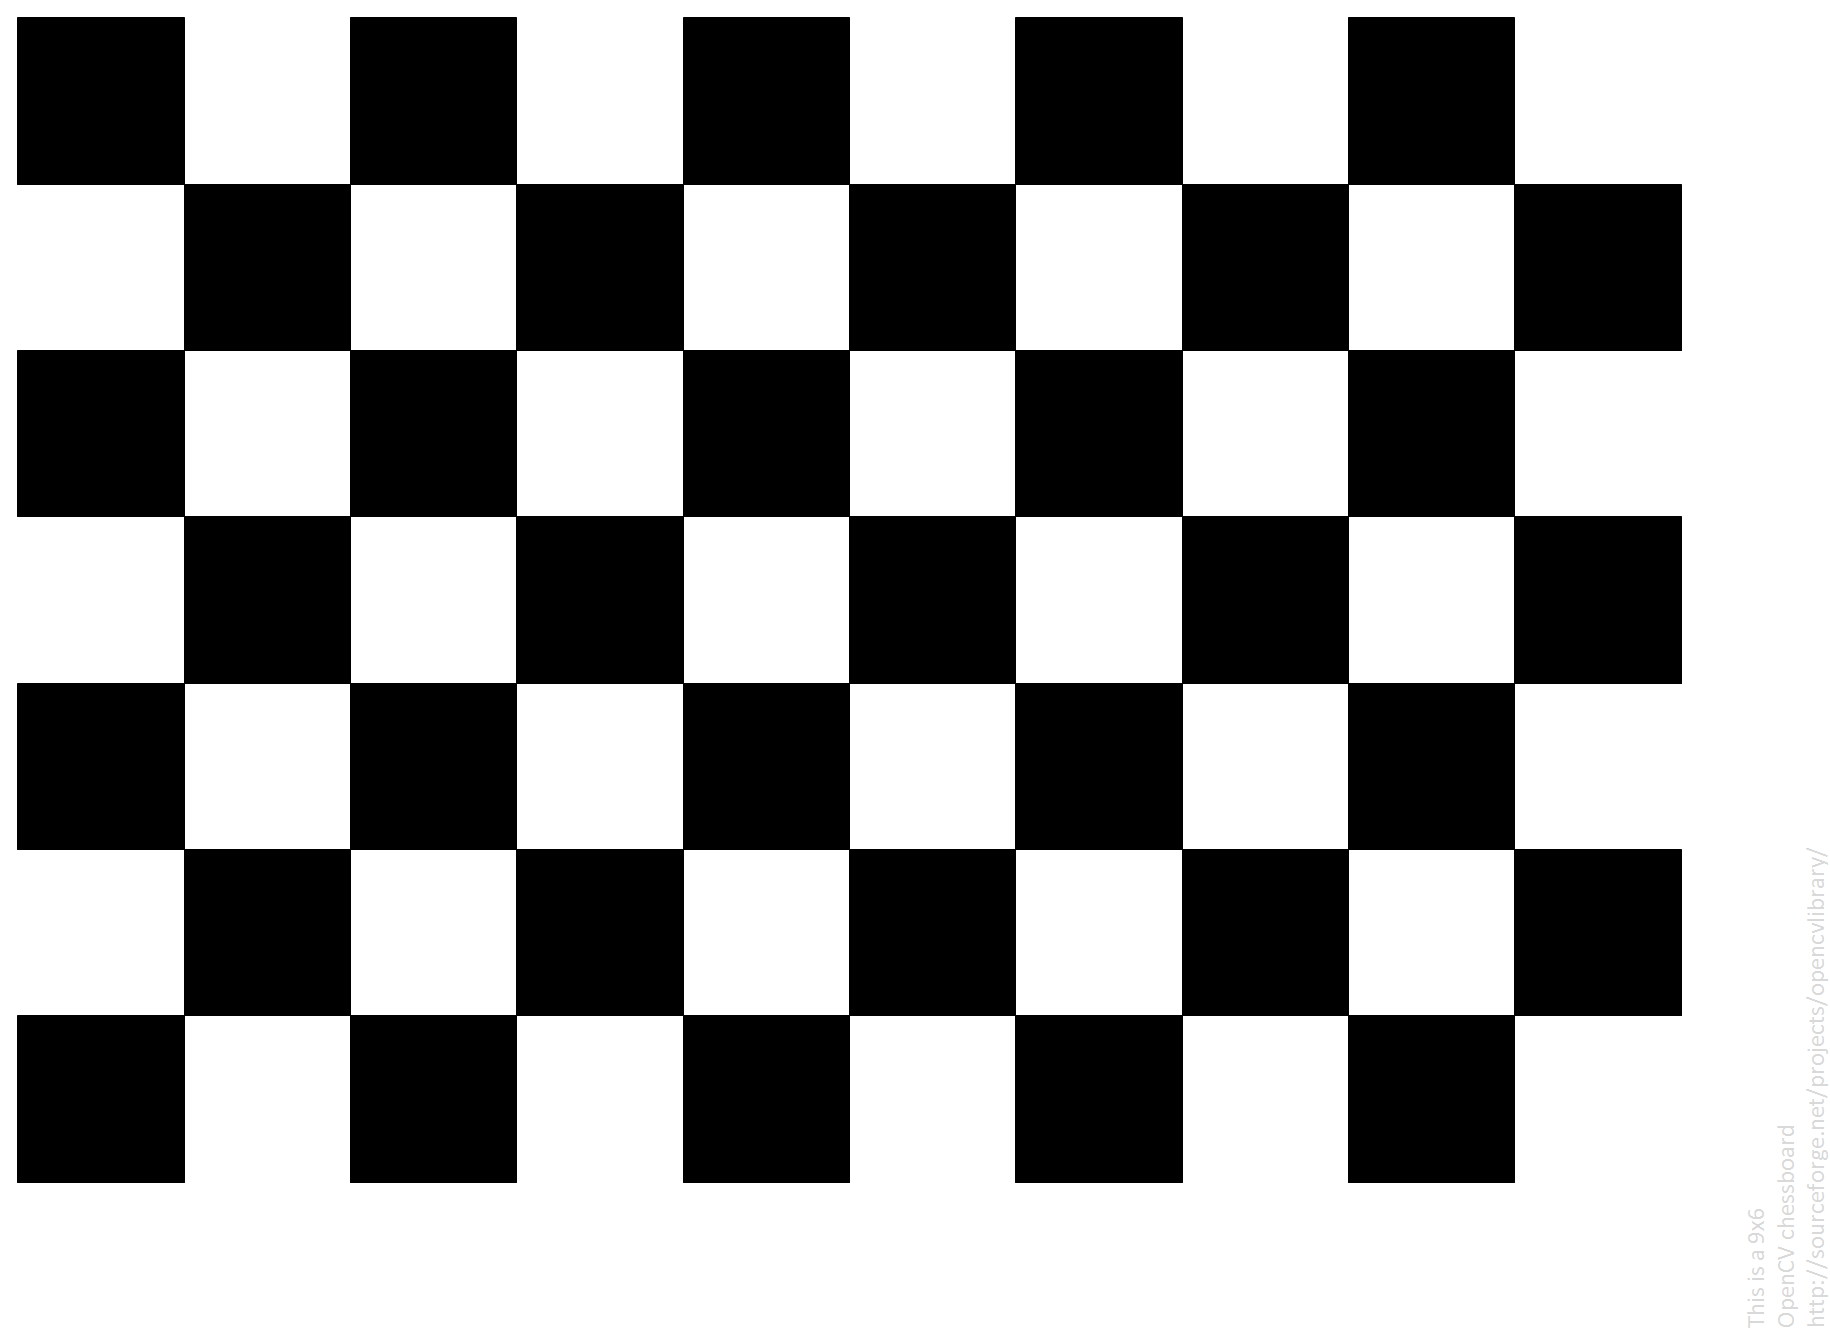
\includegraphics[width=\linewidth]{Imagens/figura3-3E3-12.png}
  \caption{Tabuleiro de xadrez}\label{fig3:3}
\endminipage\hfill
\minipage{0.32\textwidth}
  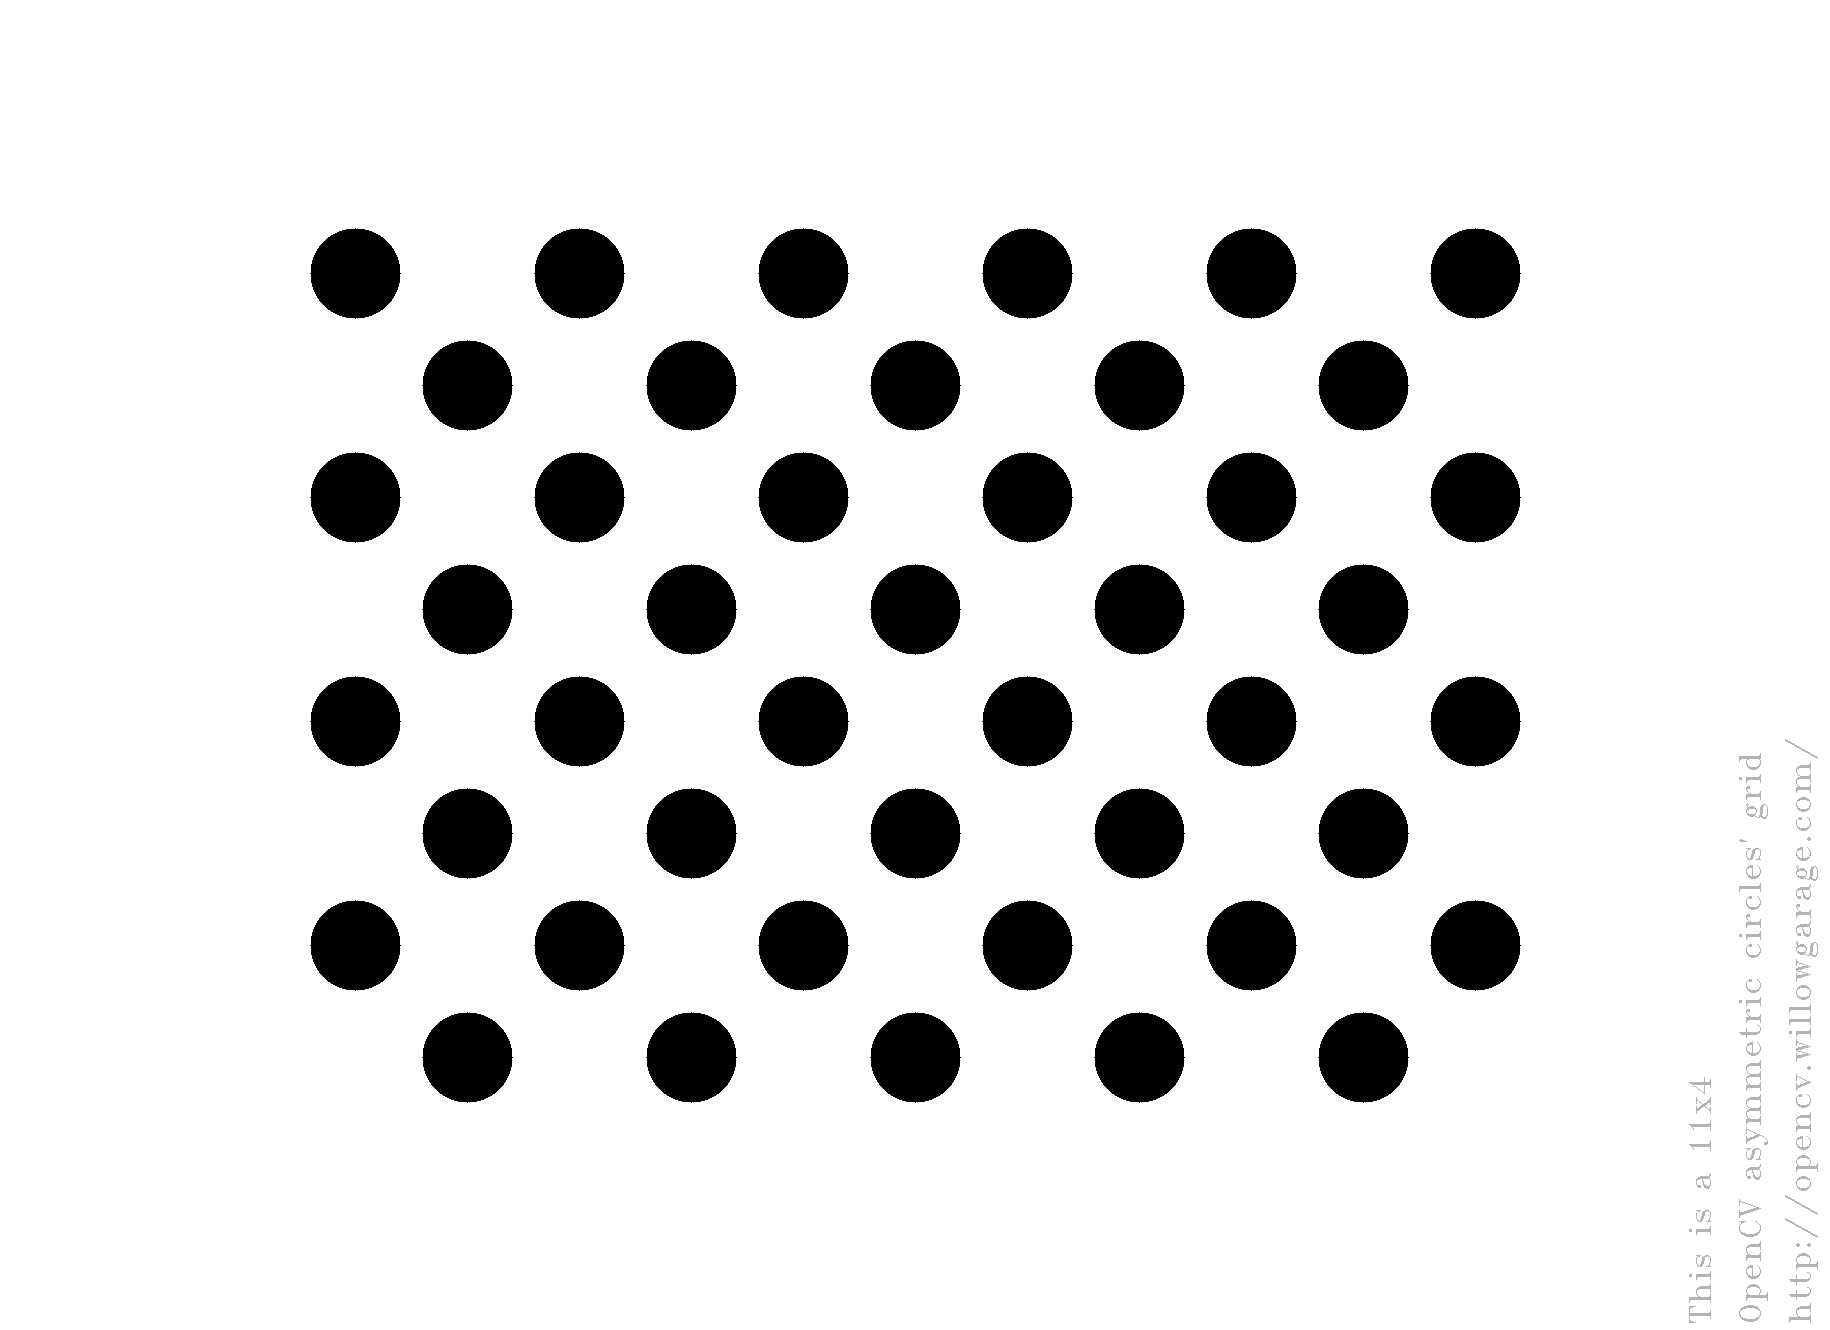
\includegraphics[width=\linewidth]{Imagens/figura3-4.png}
  \caption{Círculos alinhados assimetricamente}\label{fig3:4}
\endminipage\hfill
\minipage{0.32\textwidth}
  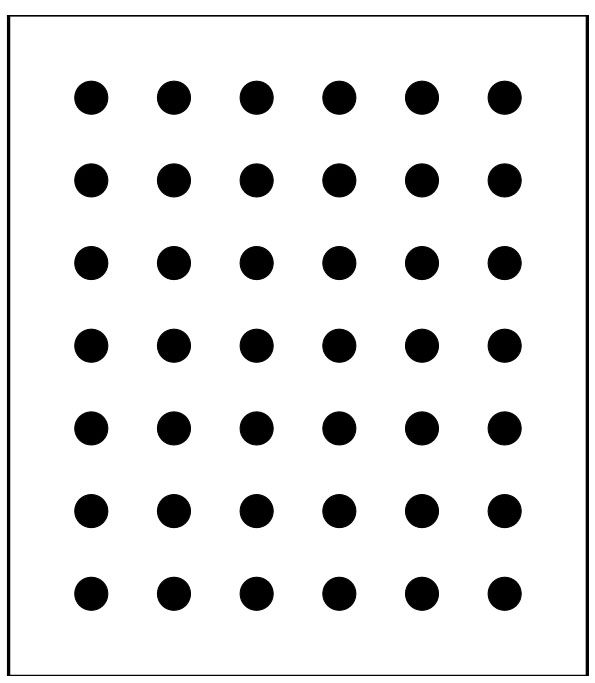
\includegraphics[width=\linewidth]{Imagens/figura3-5.jpg}
  \caption{Círculos alinhados simetricamente}\label{fig3:5}
\endminipage
\end{figure}


\begin{figure}[!hb]
\minipage{0.49\textwidth}
  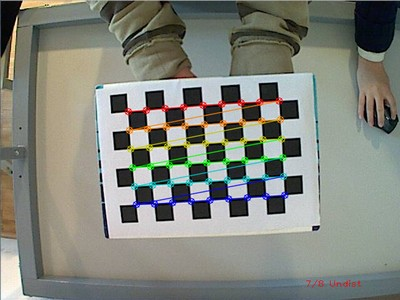
\includegraphics[width=\linewidth]{Imagens/figura3-6.jpg}
  \caption{Reconhecimento do tabuleiro de xadrez}\label{fig3:6}
\endminipage\hfill
\minipage{0.49\textwidth}
  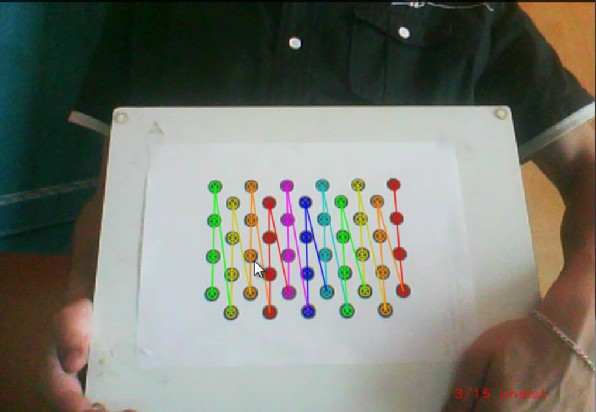
\includegraphics[width=\linewidth]{Imagens/figura3-7.jpg}
  \caption{Reconhecimento dos círculos alinhados assimetricamente}\label{fig3:7}
\endminipage
\end{figure}

Ao fim da calibração, o algoritmo retorna a matriz de calibração da câmera, a qual servirá para remover a distorção radial das imagens capturadas posteriormente; vale frisar que a distorção radial será removida somente se  a matriz de calibração tenha sido calculada corretamente. As figuras \ref{fig3:8},\ref{fig3:9},\ref{fig3:10}	 e\ref{fig3:11} mostram mais exemplos da execução do aplicativo para obter \textit{keypoints} bem como a contra partida sem filtragem:

\begin{figure}[H]
	\centering
		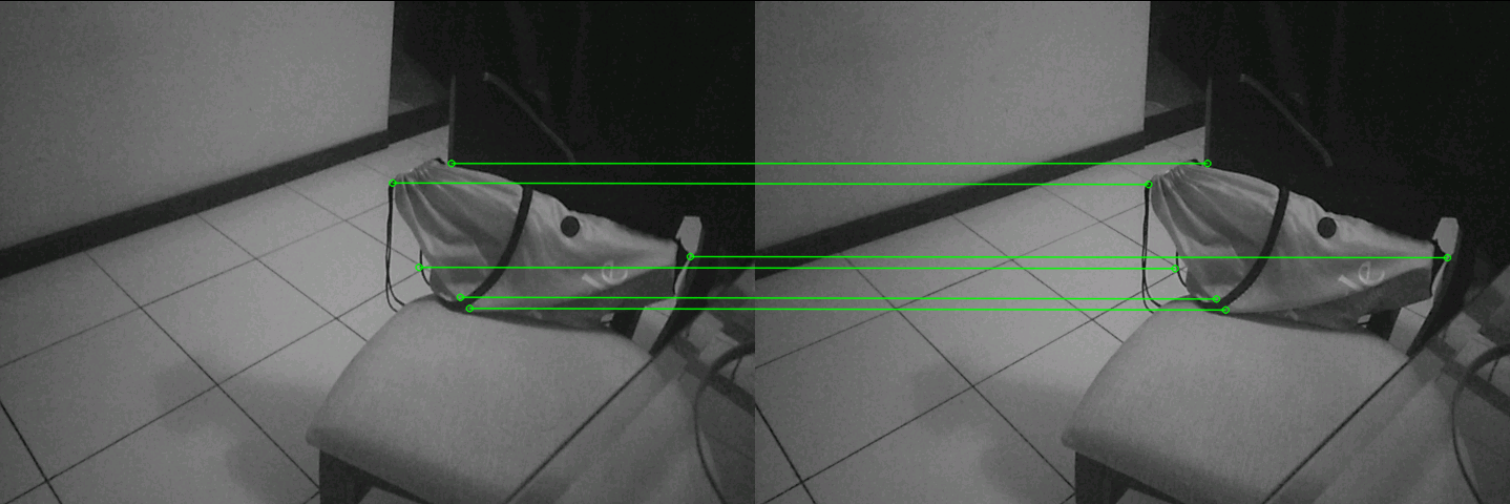
\includegraphics[width= \textwidth]{Imagens/figura3-8.png}
	\caption{Execução do \textit{PhotoGuide} e os \textit{keypoints} filtrados da cena \#1}
	\label{fig3:8}
\end{figure}

\begin{figure}[H]
	\centering
		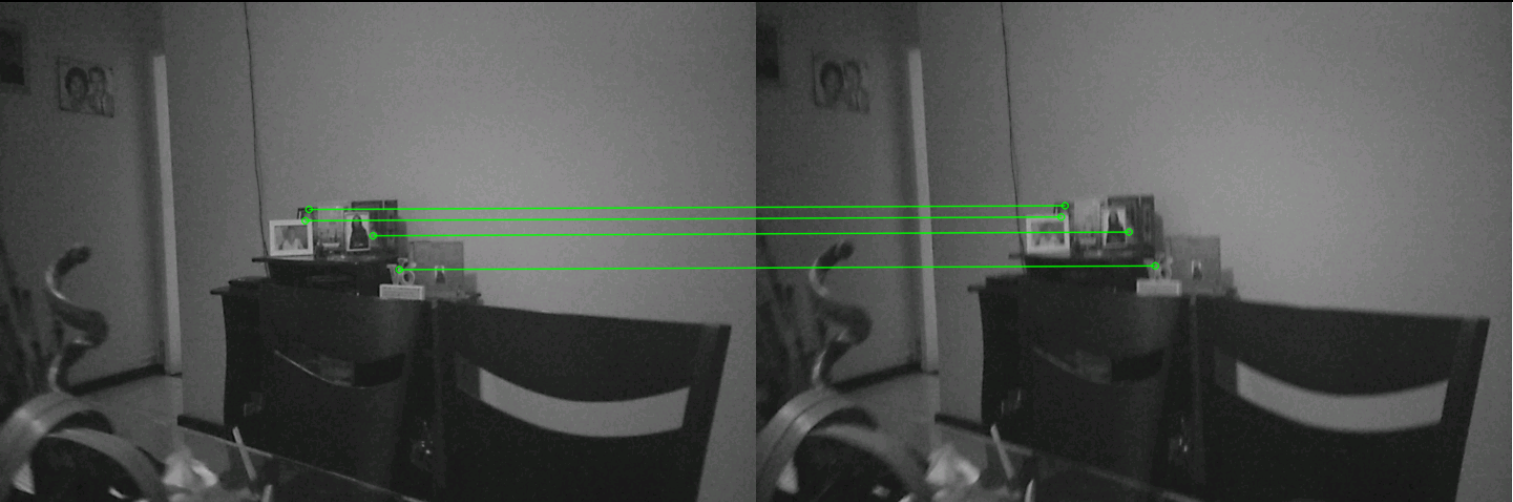
\includegraphics[width= \textwidth]{Imagens/figura3-9.png}
	\caption{Execução do \textit{PhotoGuide} e os \textit{keypoints} filtrados da cena \#2}
	\label{fig3:9}
\end{figure}

\begin{figure}[H]
	\centering
		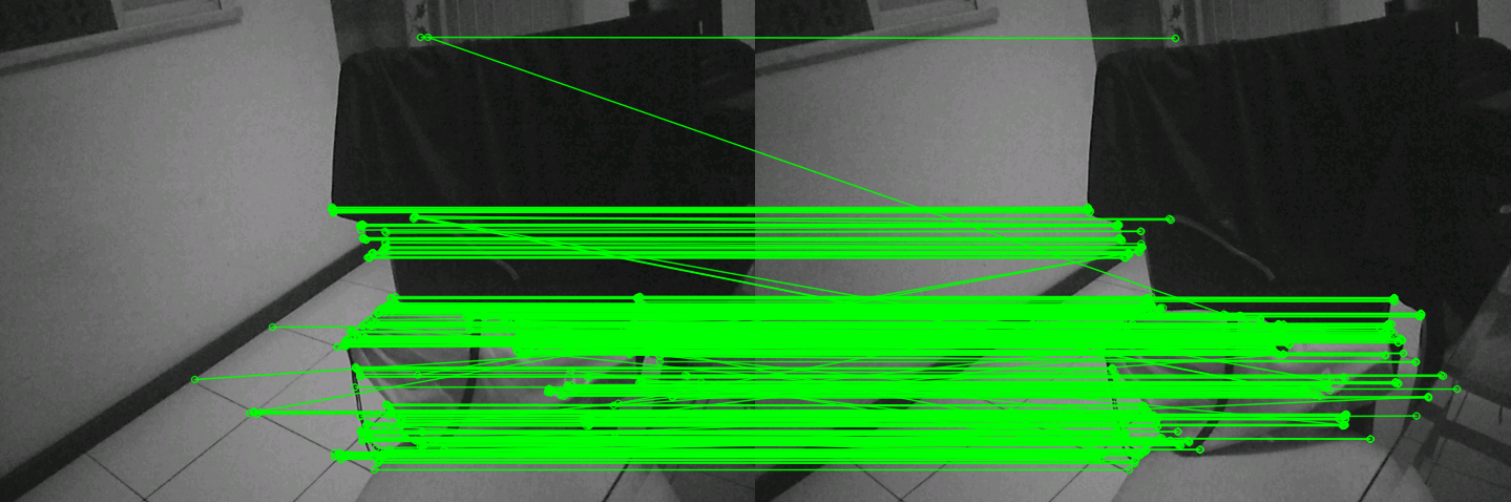
\includegraphics[width= \textwidth]{Imagens/figura3-10.png}
	\caption{\textit{Keypoints} não filtrados da cena \#1}
	\label{fig3:10}
\end{figure}

\begin{figure}[H]
	\centering
		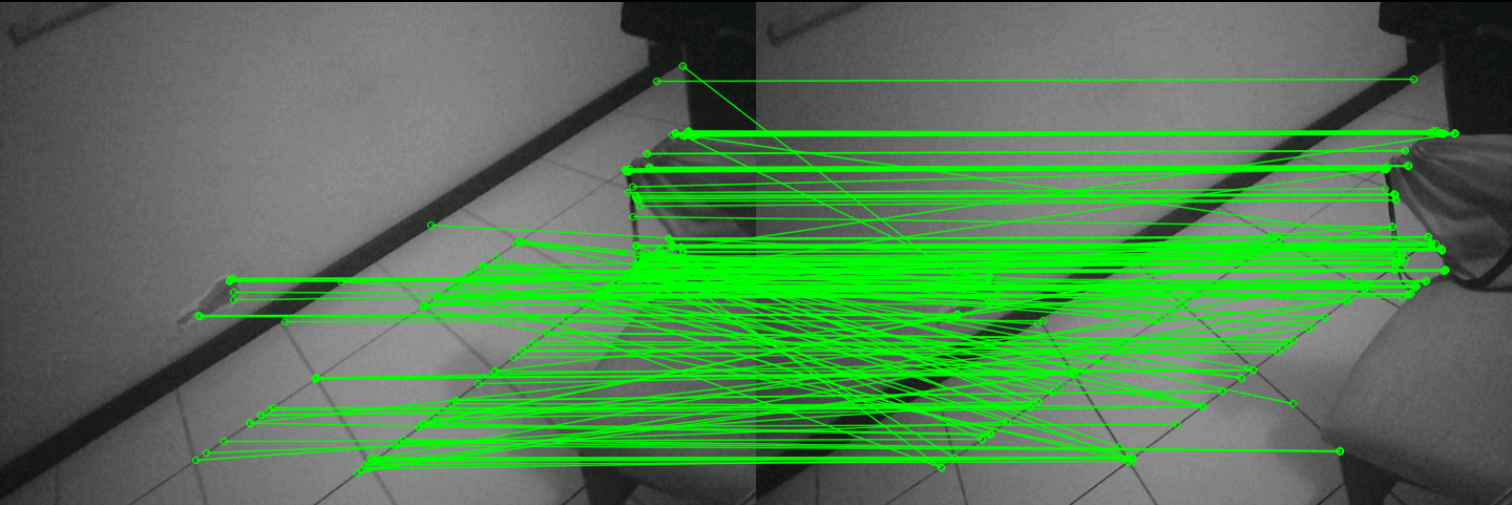
\includegraphics[width= \textwidth]{Imagens/figura3-11.png}
	\caption{\textit{Keypoints} não filtrados da cena \#2}
	\label{fig3:11}
\end{figure}


É possível perceber a importância de se detectar e remover falsos positivos, ou \textit{outliers}, já que essa quantidade de pontos errôneos afetaria drasticamente o processamento.

\subsection{Dificuldades Encontradas}

Durante o desenvolvimento do \textit{PhotoGuide}, certos problemas causaram grande dificuldade para a continuação de sua implementação. A ausência de documentação, bem como o tamanho pequeno da comunidade de desenvolvimento utilizando \textit{OpenCV} no \textit{Android} dificultam a pesquisa por casos semelhantes ou para a procura de auxílio com o código fonte, bem como a questão de que a maior parte dos resultados encontrados são escritos para a linguagem \textit{C++}, que é mais permissiva do que \textit{Java}®, a linguagem utilizada no desenvolvimento do \textit{PhotoGuide}. Outros problemas provenientes disso são as diferenças entre implementações, já que em \textit{C++}, é possível realizar diversas operações entre os tipos de \textit{Mat},  que é uma estrutura do \textit{OpenCV} para armazenar informações acerca de uma matriz, fato que não se torna possível em Java já que não foram implementados herdando de uma classe em comum. Para certas tarefas, era possível utilizar o \textit{JNI (Java Native Interface)}\cite{JNI}, que permite que código escrito em \textit{Java }realize chamadas para códigos escritos em outras linguagens, e neste deste trabalho, \textit{C++}. O \textit{JNI} é utilizado principalmente quando se é necessário utilizar uma biblioteca já implementada em outra linguagem, ou quando a complexidade do código na outra linguagem possui uma menor complexidade. No \textit{PhotoGuide}, não foram encontradas melhorias significativas utilizando \textit{JNI}. 

Outro problema encontrado foi o baixo desempenho, já que a captura constante de quadros junto ao processamento de pares se mostrou demasiadamente onerosa para serem executados num \textit{smartphone}. Tendo em vista esses problemas, optamos  apenas que a captura de quadros e vídeo fosse feita utilizando a \textit{PSEye}® e depois de um tempo usando vídeo capturado de \textit{smartphone} e extraído os seus quadros usado um \textit{software} a parte, e o processamento fosse feito numa máquina de maior poder de processamento, como um \textit{desktop} ou \textit{laptop}.

\section{\textit{LSD-SLAM}}

A abordagem seguinte adotada no projeto foi a reconstrução de ambientes utilizando o \textit{LSD-SLAM}. O \textit{LSD-SLAM} é uma ferramenta poderosa porém com pouca documentação, o uso dela se mostra trabalhoso devido ao número grande de parâmetros de configuração possíveis e condições de luz e posição, cada ambiente possui suas próprias configurações otimizadas. A capacidade dessa ferramenta de exportar seus mapas 3D em um tipo de arquivo de fácil leitura faz dela facilmente adaptada para qualquer projeto de navegação 3D e reconhecimento espacial. Aprimoramentos em usabilidade e documentação são desejadas para futuras versões dessa ferramenta caso seus desenvolvedores continuem atualizando. Nessa sessão serão discutidos particularidades de configuração, uso, funcionamento e métodos da utilização dessa ferramenta.

\subsection{Configurações utilizadas}

O \textit{LSD-SLAM} foi testado nas seguintes configurações de máquina, um desktop e um laptop, respectivamente:

\begin{itemize}
	\item{Processador	\textit{AMD FX™-8350 Eight-Core Processor}, 4000 Mhz, 4 Núcleos, 8 Processadores Lógicos}
	\item{8GB de memória \textit{RAM}}
	\item{Placa gráfica \textit{AMD Radeon R2 260x}}
\end{itemize}

e:

\begin{itemize}
	\item{Processador \textit{Intel® Core™ i3 M370}, 2399 Mhz, 2 Núcleos, 4 Processadores Lógicos}
	\item{4GB de memória RAM}
	\item{Placa gráfica integrada: \textit{Intel® HD Graphics}}
\end{itemize}	

Softwares e periféricos utilizados:

\begin{itemize}
	\item{\textit{Ubuntu} versão 14.04\cite{Ubuntu}}
	\item{Câmera \textit{PSEye®}, modelo para o \textit{console} \textit{PlayStation®} 3.}
	\item{Câmera embutida no \textit{smartphone Motorola® Moto X Play} 32GB em junção com o aplicativo \textit{OpenCamera} para \textit{Android}.}
	\item{\textit{Software VLC} para extrair os quadros dos vídeos capturados pela câmera.}
	\item{\textit{Software ROS Indigo}.\cite{ROS-Tutorial}}
	\item{\textit{Driver} para \textit{webcam} usb\_cam.\cite{Setup-USBCAM}}
\end{itemize}

No começo da utilização do \textit{LSD-SLAM} foi testada a câmera \textit{Logitech® HD Webcam c270}, porém essa câmera não oferecia a capacidade mínima recomendado pelo \textit{LSD-SLAM} para obter resultados decentes, que era ter taxa de quadros de pelo menos 30 \textit{FPS} e \textit{global shutter}, em que todos os \textit{pixels} do quadro são expostos ao mesmo tempo, a \textit{PSEye®} se enquadrava em ambos os requisitos e foi usada no lugar da \textit{Logitech}. No entanto usar a câmera \textit{PSEye®} apesar de permitir um resultado melhor, era uma câmera \textit{USB} que devido a mobilidade da câmera estava limitada ao cabo além do próprio tamanho e peso do \textit{notebook} limitava a captura de \textit{datasets} a ser feita usando um \textit{notebook} com a \textit{PSEye®} conectada. Após algum tempo usando a \textit{PSEye®}, os testes foram migrados para a câmera do \textit{smartphone Motorola® Moto X Play}, que tem como diferencial a sua captura de vídeos em mais de 30\textit{FPS} em alta taxa de \textit{bits}. Apesar da câmera não ser \textit{global shutter} e sim \textit{rolling shutter}, em que os \textit{pixels} são expostos sequencialmente em uma direção, que é mais comum entre câmeras \textit{smartphone}, o resultado for satisfatório para o objetivo do trabalho de oferecer o mapeamento 3D do ambiente a partir de um aparelho móvel. A calibração da câmera \textit{smartphone} foi obtida a partir da calibração do \textit{PhotoGuide} e usada como parâmetro para o \textit{LSD-SLAM} usando o método de conversão na sessão 3.2.3.7.

\subsection{Captura dos \textit{datasets}}

Os \textit{datasets} capturados foram os seguintes:

\begin{itemize}
	\item{Fachada do DCOMP virada para o estacionamento usando a câmera \textit{PSEye®} - 6180 imagens - 119621}
	\item{Jardim de área residencial usando a câmera \textit{PSEye®} - 660 imagens - 87093 pontos}
	\item{Sala de Mestrado II usando a câmera \textit{PSEye®} - número de imagens desconhecido por ter sido feito usando o live\_slam sem salvar as imagens - 168915 pontos}
	\item{Fachada do DCOMP virada para o estacionamento usando a câmera do \textit{smartphone Motorola® Moto X Play} 32GB- 3280 imagens - 3680087 pontos}
	\item{Corredor interno do 1º andar do DCOMP usando a câmera do \textit{smartphone Motorola® Moto X Play} 32GB - 8319 imagens  - 5877083 pontos}
\end{itemize}

Todos os datasets foram capturados a 30FPS e resolução de 640x480.

